\documentclass[preprint,12pt,authoryear]{elsarticle}

\usepackage{amsmath}
\usepackage{amsfonts}
\usepackage{amssymb}
\usepackage[utf8]{inputenc}
\usepackage{url,hyperref,lineno,microtype,subcaption}
\usepackage{color,tensor,multirow,siunitx}
\usepackage[onehalfspacing]{setspace}
\usepackage{makecell}
\renewcommand{\cellalign}{cl}
\usepackage{caption}
\captionsetup[figure]{name=Fig., labelfont=bf}
\captionsetup[table]{name=Table, labelfont=bf}
\usepackage{appendix}
\usepackage[utf8]{inputenc}
\usepackage[T1]{fontenc}
\usepackage[english]{babel}
\usepackage{changepage}
\usepackage{lineno}

\usepackage{lipsum}


\definecolor{red}{rgb}{1,0,0}
\definecolor{blue}{rgb}{0,0,0.8}
\definecolor{orange}{rgb}{1,0.5,0}
\newcommand{\emphc}[1]{\emph{\textcolor{red}{#1}}}
\newcommand{\modif}[1]{\textcolor{orange}{#1}}
\newcommand{\mean}[1]{\langle {#1} \rangle}

\newcommand{\hycom}{\textsc{hycom} }
\newcommand{\slim}{\textsc{slim}\ }
\newcommand{\ie}{{\it i.e.}\ }
\newcommand{\eg}{{\it e.g.}\ }


\journal{TDB}

\begin{document}

\begin{frontmatter}

    \title{Building a model-based coral connectivity atlas of Florida’s Coral Reef}

    \author[eli]{Thomas Dobbelaere\corref{corr}}
    \ead{thomas.dobbelaere@uclouvain.be}
    \author[nova]{Ryan Chabotte}
    \author[nova]{Joana Figueiredo}
    \author[lsu]{Daniel M. Holstein}
    \author[eli,immc]{Emmanuel Hanert}
    \cortext[corr]{Corresponding author}

    \affiliation[eli]{
        organization={Eath and Life Institute (ELI), UCLouvain},
        % addressline={},
        city={Louvain-la-Neuve},
        % postcode={1348},
        % state={},
        country={Belgium}
    }
    \affiliation[nova]{
        organization{Halmos College of Natural Sciences and Oceanography, Nova Southeastern University, United States}
        % addressline={},
        city={Dania Beach},
        % postcode={1348},
        state={Florida},
        country={USA}
    }
    \affiliation[lsu]{
        organization={Department of Oceanography and Coastal Sciences, College of the Coast and Environment, Louisiana State University},
        % addressline={},
        city={Baton Rouge},
        % postcode={1348},
        state={Louisiana},
        country={USA}
    }
    \affiliation[immc]{
        organization={Institute of Mechanics, Materials and Civil Engineering (IMMC), UCLouvain},
%        % addressline={},
        city={Louvain-la-Neuve},
%        % postcode={1348},
%        % state={},
        country={Belgium}
    }

    \begin{abstract}
        Coral populations have experienced a world-wide decline due to both global and local anthropogenic stressors and almost all live coral cover could be lost under a >1.5°C warming. Avoiding climate change being no longer an option, local actions are required to mitigate its effects and support coral recovery. To maximize the resilience of large-scale reef systems with localized actions, knowledge about the connectivity between reefs is needed. These exchange processes are driven by currents with complex small-scale circulation features within reef systems. Hence, biophysical models that can simulate the life-traits and transport of coral larvae down to the reef scale are required to estimate coral connectivity. However, due to the important computational cost of such models, connectivity studies often consider a small number of coral species over a limited number of spawning events, therefore lacking inter-annual and inter-specific variability. Here, we used the multi-scale ocean model \slim to simulate the dispersal of larvae from 6 coral species in Florida's Coral Reef over 10 consecutive years (2012-2021). We then computed connectivity metrics to identify the reefs best suited for protection and restoration efforts over multiple years and multiple species. By identifying similar spatial patterns in connectivity measures between species, we highlight the potential for coupled restoration. Furthermore, using 10 years of modeled larval dispersal, we build robust estimates of long-term connectivity. Such estimates could be used to predict the potential evolution of the reef system and bridge the gap between genetic connectivity and larval dispersal in Florida's Coral Reef. This study provides unprecedented easy-to-access reef-scale connectivity datasets to inform the  design of future marine conservation strategies.
    \end{abstract}

    \begin{keyword}
    Florida's Coral Reef \sep biophysical modeling \sep Connectivity
    \end{keyword}
\end{frontmatter}

\linenumbers

% === INTRODUCTION ===

\section*{Introduction}

Coral reefs are complex and biodiverse ecosystems that for the past decades have been facing multiple stressors and consequently declining globally. The rapid decline of coral populations is due to direct and indirect anthropogenic stressors, such as climate change, nutrient and sediment run-off, overharvesting of herbivores and pollution \citep{hughes2003climate, hughes2018spatial, hoegh2007coral, hoegh2017coral}. Increased frequency and intensity of disturbances, such as heat events and disease, decrease coral fecundity and often leads to mortality. When adult coral density is low, it becomes less likely that the eggs of a colony will meet the sperm of another colony, reducing fertilization success and consequently the number of larvae that could recruit and replenish populations. Larval settlement success and post-settlement survival and growth are also reduced due to increased sedimentation, turf and macroalgae overgrowth and high frequency of heat disturbances. As a result, many reefs around the world, such as the Florida’s Coral Reef, have lost resilience and no longer fully recover following acute disturbances \citep{jones2022frequent}.

As an infamous hot spot for coral disease, the Caribbean has already experienced a 50-80\% decline of live coral cover since the 1970s \citep{gardner2003long,jackson2014status}. Furthermore, the Caribbean is currently experiencing an outbreak of the stony coral tissue loss disease (SCTLD), one of the most pervasive and virulent coral diseases on record, which affects over 22 species of reef-building corals \citep{noaa2018,meiling2021variable}. This disease was first observed off the coast of Miami in 2014 \citep{precht2016unprecedented}, and has since then decimated coral populations throughout the entirety of Florida's Coral Reef (FCR) \citep{williams2021fine,frrp2021}. As a consequence, coral cover in Southeastern Florida has now dropped below 1\%, while reefs in the Florida Keys maintained a cover of roughly 6\% \citep{grove2022national}. However, extreme warm events have increased significantly in the Florida Keys in recent decades and, if trends persist, annual bleaching could occur in the region before 2034 \citep{manzello2015rapid}. Besides, Florida is a prime landfall target for tropical cyclones, which are expected to increase in intensity under climate change. It becomes thus urgent to maintain coral populations and support their recovery through restoration and conservation efforts.

Connectivity-informed coral restoration can directly repopulate small reef areas but also indirectly promote natural processes of recovery (sexual reproduction and recruitment). When genetically different corals are outplanted on the reef in close proximity, it increases the chances their gametes will get fertilized \citep{omori2019coral}. Moreover, if the sites which due to local currents distribute the larvae produced to a greater number of (farther, unrestored) reefs (termed source reefs, \citealp{bode2018resilient}) were prioritized for restoration \citep{king2023larval}, it would hasten reef recovery and resilience to disturbances. Reef connectivity, and thus the location of source reefs within a reef system, can be determined using bio-physical models of coral larval dispersal \citep{frys2020fine, figueiredo2022global,king2023larval}. These models use high-resolution (multi-year) ocean circulation dynamics and empirically calibrated larval dynamics, specifically larval survival (how long larvae remain alive for) and competency (when larvae become ready to settle and metamorphose into a coral polyp and when this ability is lost), to predict larval dispersal and settlement within a reef system. The problem is that the larval dynamics for most Caribbean corals, necessary to build these models, remains to be described.

Understanding reef connectivity is also important to determine where to place marine protected areas, identify areas which are more vulnerable to disturbance (fewer chances to be rescued), and areas which are more resilient (well-connected). Inter-specific differences in larval survival and competency determine the species’ tendency to either settle on their natal reef (local retention, a measure of reef’s self-persistence) and/or disperse long-distances, potentially recolonizing distant reefs thus increasing the connectivity and genetic diversity of its populations. At the reef level, having high levels of local retention (proportion of larvae produced by a reef that settled back on that reef) means this reef has a higher ability of self-replenishment. If a reef has high self-recruitment (proportion of the settlers on a reef that originated from larvae produced on that reef) it means it is highly isolated.  Although more shielded from human influence, isolated reefs are more susceptible to larger perturbations such as severe storms or oil spills \citep{baumann2022remoteness} because if disturbed they are rarely replenished by larvae coming from other locations. Sink reefs i.e., reefs which receive larvae from many other reefs, have a high network persistence and are expected to recover faster following disturbances. Source reefs are optimal locations for marine resource managers to prioritize for protection; the preservation of source reef through marine reserves or marine protected areas ensures larval supply at both local and regional scales \citep{muenzel2023integrating}, contributing to the resilience of entire reef system.

\emphc{Add some transition sentences here}. Such models require important computational resources and most connectivity studies cover thus a limited number of spawning events and coral species. This undermines the robustness of the derived connectivity estimates, as they lack inter-annual and interspecific variability. In this study, we simulated the dispersal of larvae from 6 coral species over 10 consecutive years (2012-2021). Using these 10 years of simulation, we identify consistent connectivity hotspots and clusters for all simulated years and species. Furthermore, by identifying pairs of coral species with strongly correlated connectivity metrics, we highlight the potential for coupled management strategies.

% === METHODS ===

\section*{Methods}

\subsubsection*{Larval survival and competency dynamics}

% \emphc{(Sihould probably move stuff to appendix)} We experimentally calibrated the larval survival and competency of six Caribbean coral species, \textit{Diploria labyrinthiformis}, \textit{Acropora cervicornis}, \textit{Pseudodiploria strigosa}, \textit{Colpophyllia natans}, \textit{Montastraea cavernosa}, and \textit{Orbicella faveolata}.This species were selected because they are key reef-building species that were severely affected by SCTLD. Larvae were obtained through successful induction of gonad maturation and synchronous spawning ex situ at Nova Southeastern University, Florida Aquarium, and University of North Carolina Wilmington.  Montastraea cavernosa was the only gonochoric species studied. Sperm was collected using a 25 mL pipette, ensuring the necessary higher concentration of sperm for fertilization \citep{fogarty2012asymmetric, fogarty2012weak, dela2020optimising}. Eggs were collected at the surface of the water and mixed with the sperm in bowls for fertilization. All the other species were hermaphroditic and thus released both eggs and sperm in bundles. Bundles were collected at the surface of the water and put into fertilization bowls. As bundles dissociated, seawater was added to the bowls to attain the sperm concentration close to 106 sperm cells/mL known to maximize fertilization \citep{fogarty2012asymmetric, fogarty2012weak, dela2020optimising}. Fertilization success was confirmed about one to one and a half hours after pooling the gametes by observing embryos undergoing cell division. Embryos were then promptly washed two to three times to remove unused sperm, using a gravy separator to ensure a clean culture. \textit{A. cervicornis} gametes were collected from colonies which sexually matured on the reefs off Fort Lauderdale, FL (USA), and brought to the outdoor aquaria for spawning a few days before their expected spawning time. \textit{O. faveolata} gametes were obtained from colonies at Biscayne Bay National Park. The other species were kept in aquaria year-round and induced to mature their gonads and spawn in the lab by mimicking natural cycles of light and temperature. To assess larval survival over time, after confirmation of fertilization, 400 fertilized embryos were collected and randomly assigned to one of four separate 200 mL glass jars each containing 100 embryos. Jars were kept on a water bath equipped with a thermostat and a small circulation pump to maintain temperature constant at 28°C. Salinity and temperature were monitored and maintained daily. All larvae were counted daily under a microscope to record the proportion of larvae alive over time. Every day for each species, water in the jar was exchanged and larvae were washed using clean seawater and placed into a clean jar. Survival experiments ended once all larvae had died. To assess larval competency over time, once the larvae of each species were observed rotating, ca. 3,500 larvae were randomly divided into three bowls. Bowls were kept in a water bath equipped with a thermostat and a small circulation pump to maintain temperature constant at 28°C and monitored daily. Aeration was added to each individual bowl to prevent settlement within the bowl and avoid anoxic conditions. The larvae in the bowls were washed daily over a filter using clean seawater. After washing, larvae were placed into clean bowls in the water bath. Daily, 40 larvae from each species were collected at random and divided evenly into four separate 200 mL glass jars that contained one pre-conditioned aragonite tile that had crustose coralline algae sprinkled upon it. After 24 hours, the tile in each jar was examined under the microscope to assess the number of larvae that had settled and metamorphosed. This process was repeated daily; larvae that remained swimming at the end of each day were not reused in the competency trials. Competency trials were completed once all larvae of a species had died in the survival trials. Larval survival and competency dynamics for each species were modelled using the methodology described by \cite{figueiredo2022global}, detailed methods in their online supplementary information.

We experimentally calibrated the larval survival and competency of six Caribbean coral species: \textit{Diploria labyrinthiformis}, \textit{Acropora cervicornis}, \textit{Pseudodiploria strigosa}, \textit{Colpophyllia natans}, \textit{Montastraea cavernosa}, and \textit{Orbicella faveolata}. These species were selected due to their significance as key reef builders and their severe impact from SCTLD. Larvae were obtained through successful induction of gonad maturation and synchronous spawning ex situ at various at Nova Southeastern University, Florida Aquarium, and University of North Carolina Wilmington. \textit{M. cavernosa}, the only gonochoric species studied, had sperm collected using a 25 mL pipette, ensuring the necessary higher concentration of sperm for fertilization \citep{fogarty2012asymmetric, fogarty2012weak, dela2020optimising}. Eggs were collected from the water surface and mixed with the sperm for fertilization. Hermaphroditic species released both eggs and sperm in bundles. Bundles were collected at the surface of the water and put into fertilization bowls with seawater to attain the concentration of 106 sperm cells/mL known to maximize fertilization \citep{fogarty2012asymmetric, fogarty2012weak, dela2020optimising}. Fertilization success was confirmed by observing embryos undergoing cell division. Embryos were then washed to remove unused sperm and ensure a clean culture. \textit{A. cervicornis} gametes were collected from sexually mature colonies off Fort Lauderdale, while \textit{O. faveolata} gametes were obtained from Biscayne Bay National Park. The other species were kept in aquaria year-round and induced to spawn in the lab. To assess larval survival, 400 fertilized embryos were equally distributed into four 200 mL jars at a constant temperature of 28°C, and monitored daily under a microscope. The water was exchanged daily, and larvae were washed and placed into clean jars until all had died. For larval competency, once larvae were observed rotating, ca 3,500 larvae were randomly divided into three bowls kept at a constant temperature of 28°C and aerated to prevent settlement and anoxic conditions. Daily, 40 larvae from each species were placed into jars with aragonite tiles with crustose coralline algae, and checked for settlement and metamorphosis after 24h using a microscope. Competency trials were repeated daily until all larvae had died. Larval survival and competency dynamics for each species were modelled using the methodology described by Figueiredo et al. (2022), detailed methods in their online supplementary information.



\subsection*{Larval dispersal and connectivity modeling}

We simulated the hydrodynamics over the entirety FCR during 10 years (2012-2021) with the multiscale ocean model \slim\footnote{\href{ https://www.slim-ocean.be}{slim-ocean.be}}. This model has already been successfully validated and applied in Florida to simulate the dispersal of larvae and disease agents \citep{frys2020fine,dobbelaere2020coupled}. \slim uses an unstructured mesh whose resolution can be locally refined in order to capture flow features and tides down to the reef scale (Fig. \ref{fig:mesh}). The model mesh was generated using the seamsh\footnote{\href{https://pypi.org/project/seamsh/}{https://pypi.org/project/seamsh/}} Python library, based on the open-source mesh generator GMSH \citep{geuzaine2009gmsh}. It was made up of $6,6\times 10^5$ triangles, whose size ranged from 50 m near reefs to 13.5 km in the open sea. The mesh element size was refined based on the distance to reefs and coastlines, as well as the bathymetry and bathymetry gradient. \slim currents were relaxed towards the operational Navy HYbrid Coordinate Ocean Model (\hycom; \citealp{chassignet2007hycom}) following the approach of \citep{dobbelaere2022impacts} to capture the baroclinic dynamics of the Florida Current. Further details about the model formulation can be found in \citep{frys2020fine}.

\begin{figure}
    \centering
    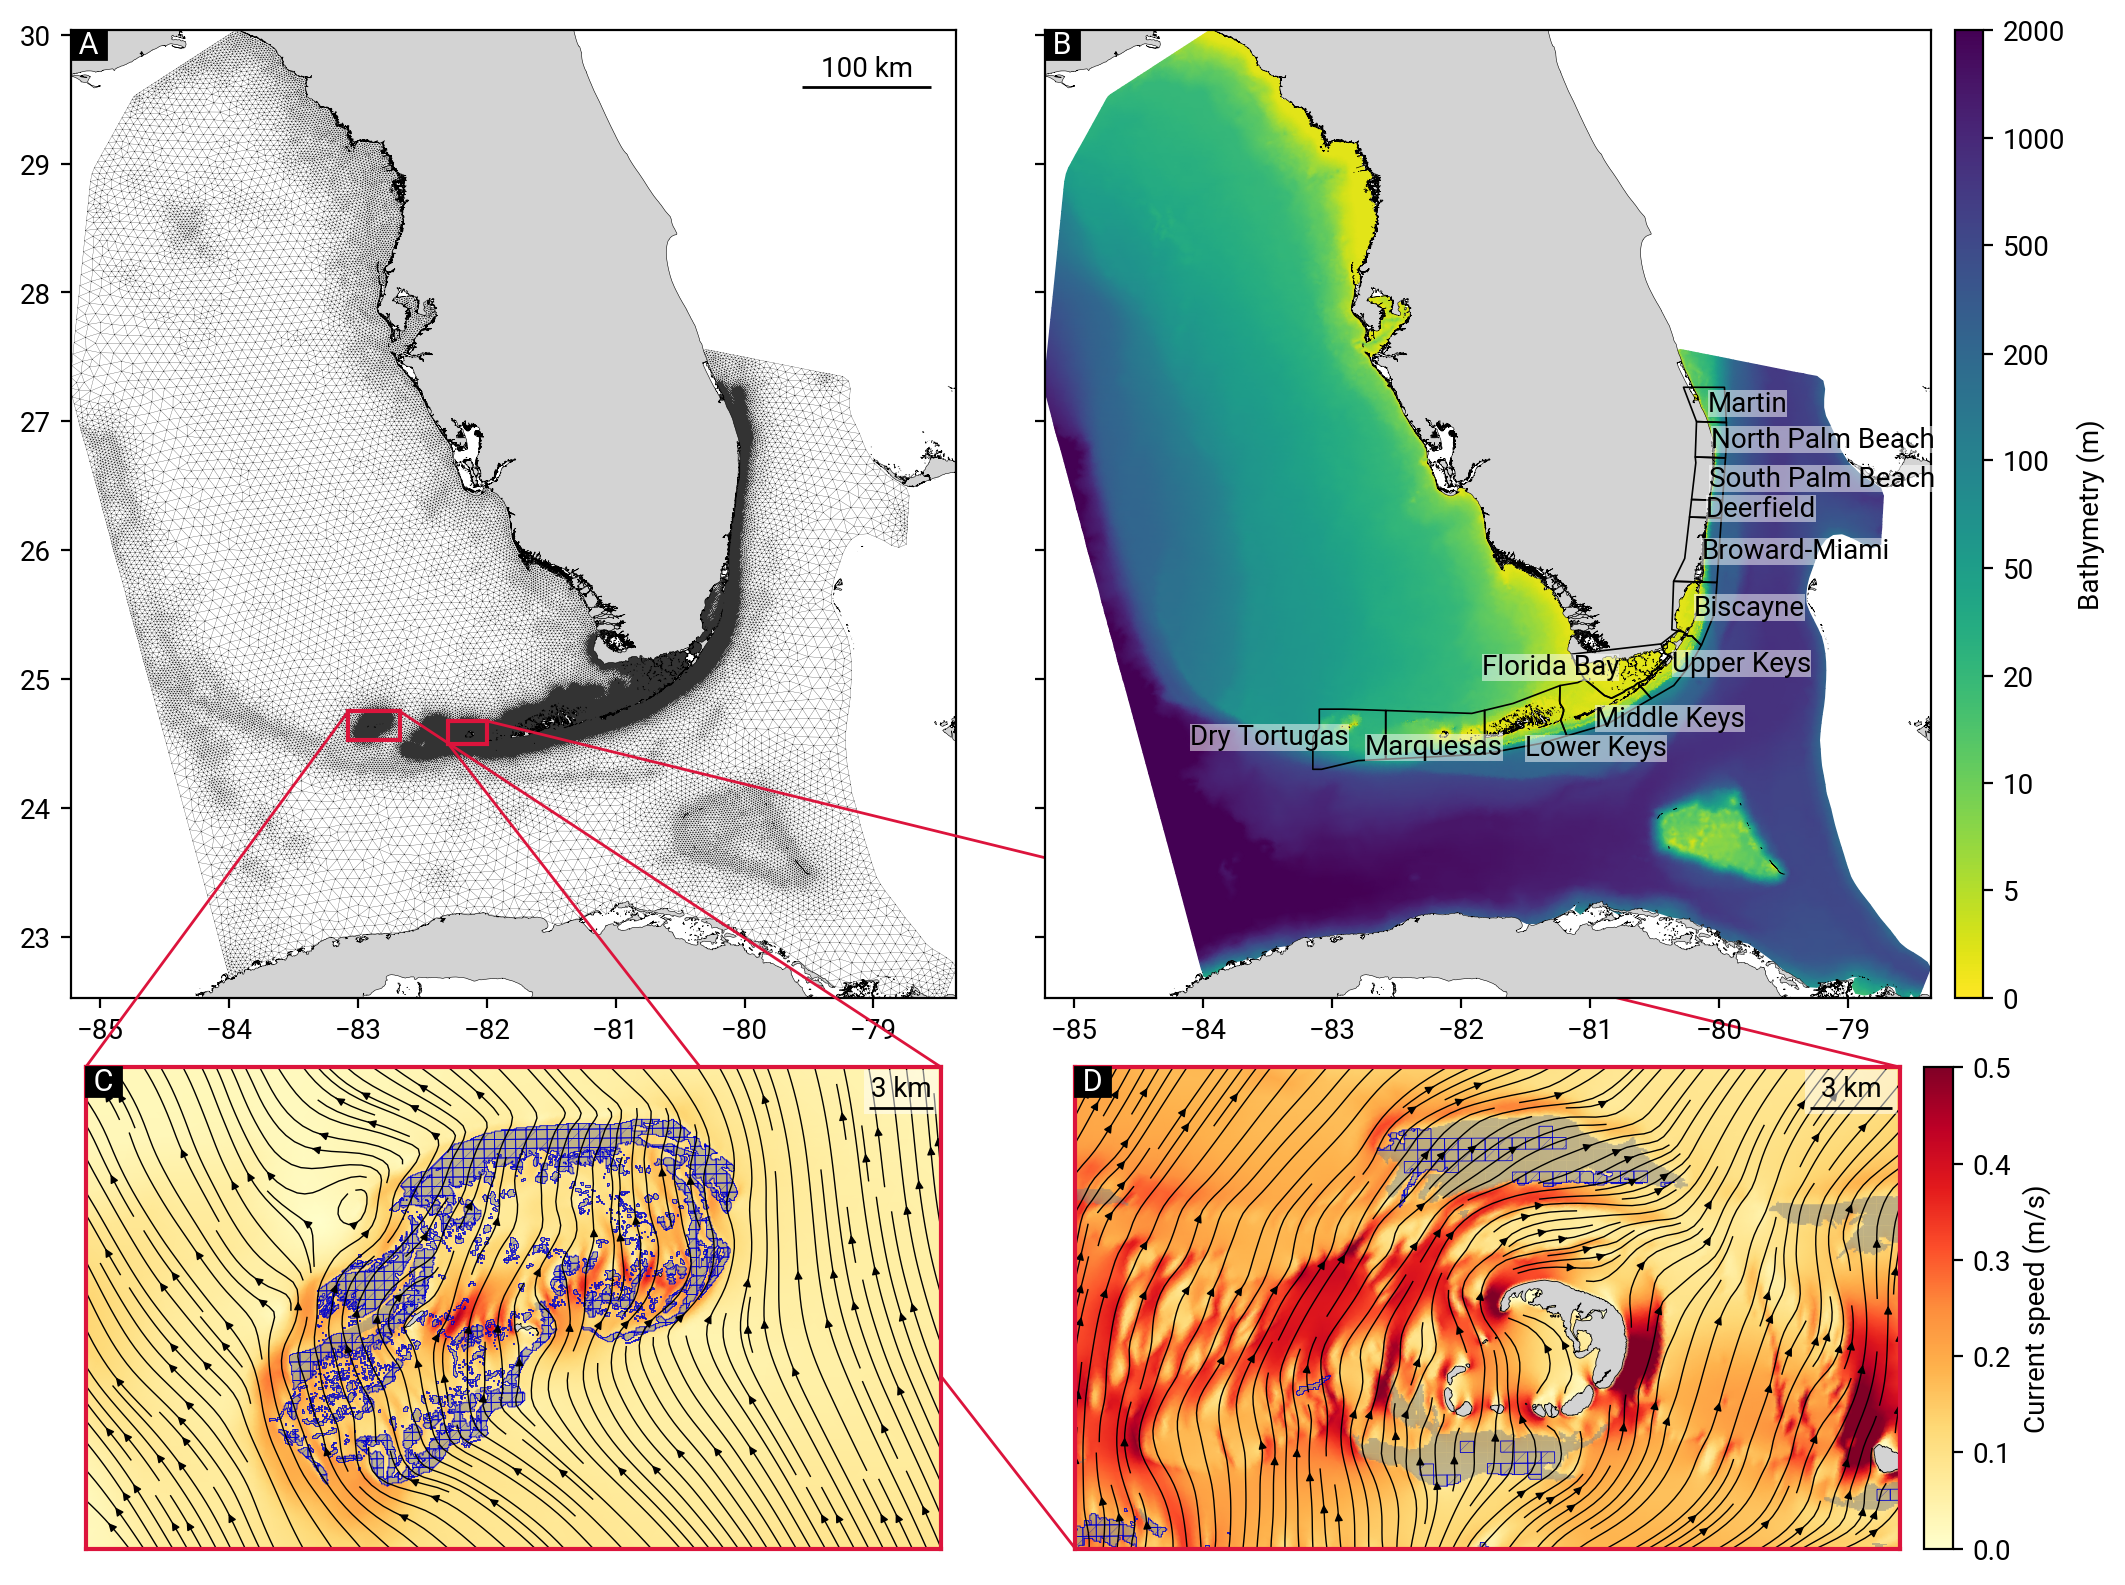
\includegraphics[width=\textwidth]{figures/fig_mesh_tnc.png}
    \caption{Model mesh (\textbf{A}) and bathymetry (\textbf{B}) with close-up views of the simulated currents in the Dry Tortugas (\textbf{C}) and the Marquesas Keys (\textbf{D}). The different regions of Florida's Coral Reef, as defined in the Unified Reef Map are shown in panel (\textbf{B}). This illustrates the ability of the model to capture complex fine-scale flow patterns near reefs and islands. Land is shown in light grey, reefs in dark grey, and reef sub-regions with live corals are highlighted in blue.}
    \label{fig:mesh}
\end{figure}
The modeled currents and the experimentally calibrated larval survival and competency were then used to simulate the larval dispersal of \textit{A.~cervicornis}, \textit{C.~natans}, \textit{D.~labyrinthiformis}, \textit{M.~cavernosa}, \textit{O.~faveolata}, and \textit{P.~strigosa}.  Larval dynamics were implemented through mortality and competence, \ie~the ability of a larvae to settle onto a reef. Mortality was modeled using a Weibull model \citep{king2023larval} with parameters $\lambda$ and $\nu$. After time to competence $t_c$, larvae were becoming competent width rate $\alpha$ and losing competence at rate $\beta$. The species-specific spawning dates and times were defined in days after the full moon (DAFM) and minutes after sunset (MAS) \textcolor{red}{[insert data source]}. \textit{D.~labyrinthiformis} spawned in April and May, \textit{M.~cavernosa} in July and August, and all other coral species spawned in July and/or August.
\emphc{I know this is the info I sent you in 2022 because it had been what was reported. The needle of info has moved a bit more now though. We now know that aside from Dlab (after April and/or May moon) and Mcav (after July and August moon), all the others are more after full moon of August and/or September spawners. They can spawn after the July moon but only if the moon is very late in July, often meaning that they spawn already in August, because they spawn about a week later. Not sure what the best way forward is as I understand this affects your simulations. We can always keep it and see if the reviewers notice it. The days of spawn after the full moon still match our knowledge and we are confident on it. For the minutes after sunset (MAS), the best reference is CARMABI tables for spawning predictions for the Southern Caribbean \url{https://www.researchstationcarmabi.org/predictions-for-coral-spawning-events-in-the-southern-caribbean-for-2022/} The actual time they spawn is different from Florida because their sunset occurs at a different time, but the MAS are consistent throughout the Caribbean.. For month of spawning, CARMABI predictions are not good for Florida because at their latitude corals spawn later in the season. There is no published summary of spawning months for Florida. We have just been gathering that information in the latest years, so maybe we can use personal observations.}

\begin{table}
    \begin{adjustwidth}{-1in}{-1in}
    \centering
    \scriptsize
    \begin{tabular}{lccccccc}
        \hline
        Species & DAFM  & MAS      &  $\lambda$     & $\nu$ & $t_c$  & $\alpha$      & $\beta$ \\
                & [day] & [minute] &  [hour$^{-1}$] & [-]   & [hour] & [hour$^{-1}$] & [hour$^{-1}$] \\
        \hline
        \textit{A.~cervivornis} & 2 - 4 & 150 - 180 & 0.005123971 & 1.303439 & 156.0769 & 0.008409655 & 0.05612717 \\
        \textit{C.~natans}      & 6 - 8 & 25 - 115  &  0.005621361 & 1.096544 & 28.20409 & 0.003140281 & 0.04740285 \\
        \textit{D.~labyrinthiformis} & 10 - 12 & -70 - 10 & 0.006276354 & 1 &  44.99998 & 0.003375632 & 0.01651378 \\
        \textit{M.~cavernosa}   & 5 - 8 & 15 - 225 & 0.002716095 & 1.49904 & 118 & 0.002647409 & 0.0337848 \\
        \textit{O. faveolata}   & 5 - 8 & 185 - 255 &  0.004567343 & 1.275355 & 108 & 0.001323208 & 0.04444537 \\
        \textit{P. strigosa}    & 6 - 8 &  35 - 100, 205 - 270 & 0.007488953 & 1.632956, & 36.01622 & 0.02547463 & 0.1775446 \\
        \hline
    \end{tabular}
    \end{adjustwidth}
    \caption{Biological and spawning parameters used to simulate the dispersal of larvae for each modeled species: days after the full moon (DAFM), minutes after sunset (MAS), Weibull model parameters for mortality ($\lambda$,$\nu$), time to competence ($t_c$), competence acquisition ($\alpha$) and loss ($\beta$) rates. The mortality rate at larval age $t$ was given by $\lambda\nu(\lambda t)^{\nu-1}$.}\label{tab:species}
\end{table}

The reefs of Florida were extracted from the “coral reefs and hardbottom” layer of the Unified Florida Reef Tract Map \citep{fwc2017unified}. The extracted reef polygon were then further divided into 16,823 500 m $\times$ 500 m sub-reef patches to model larval exchanges at a finer scale (Fig. \ref{fig:mesh}). \emphc{How did TNC select the reefs with live coral cover in the shape file ?} We assumed a uniform coral cover over all reefs, and released a total of about $10^6$ particles over all the reef polygons during each spawning simulation. Particles in the model were not representing single larvae but rather a mass of larvae, initialized at 1. Settlement of competent larval mass onto reef was occurring at deposition rate $\gamma = 0.2$ hour$^{-1}$, consistent with observed larval settling velocity \textcolor{red}{[to be confirmed]}. For each modeled spawning, the exchanges of larval mass between reefs were recorded into connectivity matrices, whose rows correspond to source reefs and whose columns correspond to destination reefs. Connectivity matrices can be more easily interpreted as large networks whose nodes are the reefs and whose edges are the larval exchanges between reefs. Connectivity metrics can then be derived from these networks using graph theory tools. The connectivity indicators used in this study are summarized in Table \ref{tab:indicators}. Finally, we identified reef clusters inside the connectivity networks using the \textit{Strongly Connected Components} (SCC) detection algorithm \citep{nuutila1994finding}. This method groups reefs in the same community if they present numerous bidirectional connections to each other, and if they are weakly connected to reefs located in other clusters. Such methods aim at identifying ecologically separated groups, hence inferring the presence of dispersal barriers between those groups \citep{thomas2014numerical,saint2023biophysical}

\begin{table}
    \begin{adjustwidth}{-1in}{-1in}
    \centering
    \small
    \begin{tabular}{p{0.25\textwidth}p{0.45\textwidth}p{0.25\textwidth}}
        \hline
        \textbf{Indicator} & \textbf{Description} & \textbf{What it shows} \\
        \hline
        %Weighted connectivity length ($WCL_i$) & $\dfrac{\sum_{j} \tilde{C}_{ij} L_{ij}}{\sum_{j} \tilde{C}_{ij}}$ & Average dispersal distance from origin to destination reef for all particles released over a reef  \\
        Weighted out-degree & Weighted combination of the number of reefs to which a given reef sends larvae and the probability of larval export to those reefs & Reef's potential to export larvae \\
        Weighted in-degree & Weighted combination of the number of reefs from which a given reef receive larvae and the probability of larval imports from these reefs & Reef's potential to import larvae \\
        Self recruitment & Proportion of particles settling on a reef that originated from that same reef. & Reef isolation \\
        Local retention & Proportion of particles released on a given reef that settle on the same reef & Self-replenishment potential \\
        \hline
    \end{tabular}
    \end{adjustwidth}
    \caption{Connectivity indicators used to analyze the dispersal of coral larvae in the reef network.}\label{tab:indicators}
\end{table}

\subsection*{Connectivity analysis}

We estimated the similarity of the distribution of the connectivity metrics between species using the Pearson correlation coefficient following the methodology described in \citep{boccaletti2014structure}. Let $x_i^\alpha$ and $x^\beta_i$ be the connectivity metrics $x$ evaluated at node $i$ for species $\alpha$ and $\beta$, the Pearson correlation coefficient between species $\alpha$ and $\beta$ for indicator $x$ is given by:
\begin{equation}
   r_{\alpha\beta} =  \dfrac{\mean{x_i^{\alpha}x_i^{\beta}} - \mean{x_i^\alpha}\mean{x_i^\beta}}{\sqrt{\mean{x_i^\alpha x_i^\alpha} - \mean{x_i^\alpha}^2}\sqrt{\mean{x_i^\beta x_i^\beta} - \mean{x_i^\beta}^2}},
\end{equation}
where $\mean{x_i}$ is the mean of sequence $\{x_i\}$. The value of $r_{\alpha\beta}$ ranges from -1 to 1, where 1 indicates a perfect positive correlation, 0 no correlation and -1 a perfect negative correlation.

For each species and indicator, we identified connectivity hot spots that remained consistent over the 10 simulated years. To do so, we evaluated the frequency at which the yearly value of each indicator was among the yearly top 10\% values of that indicator for all reefs. Reefs with a top 10\% frequency of 1 for a given indicator where thus found in the yearly top 10\% for that indicator every simulated year. By averaging this frequency for all species, we can identify hot spots that remained consistent for all simulated species and years for a given indicator. These species-averaged frequencies can then be multiplied to select optimal restoration sites. Such reef sites could be identified among top performers of weighted out-degree, in-degree and local retention, and low-performers of self-recruitment.

Finally, we assessed the inter-annual variability of the connectivity based on the connectivity indicators and the structure of the communities in the connectivity networks. We evaluated the variability of the connectivity indicators by computing the quartile coefficient of dispersion of each indicator at each reef. The formula of the quartile coefficient of dispersal writes $(Q_3-Q_1) / (Q_3+Q_1)$, where $Q_1$ and $Q_3$ are the first and third quartiles respectively. Furthermore, we quantified the inter-annual variability of the SCC structure for all species. This was performed by counting the number of simulated years during which any given pair of reefs was found in the same SCC. This resulted in a symmetrical matrix of shape \emphc{$10,055 \times 10,055$}, whose entries ranged between 0 and 10. Entries of this matrix with high values indicate pairs of reefs that were consistently found in the same SCC over the 10 simulated years. Lower values of this indicator for all reef pairs would hence infer a strong inter-annual variability of the composition of the SCCs.

% === RESULTS ===

\section*{Results}

% Indicator Mean correlation    Standard deviation
% locRet    0.652   0.143
% wInDeg    0.901   0.054
% wOutDeg   0.792   0.090
% selfRec   0.347   0.108
%
% Species 1 Species 2   Mean correlation
% Cnat  Pstr    0.875
% Mcav  Ofav    0.830
% Cnat  Ofav    0.754
% Cnat  Mcav    0.728
% Acer  Ofav    0.719
% Acer  Mcav    0.683
% Acer  Cnat    0.664
% Cnat  Dlab    0.658
% Ofav  Pstr    0.643
% Mcav  Pstr    0.608
% Dlab  Pstr    0.608
% Dlab  Ofav    0.599
% Dlab  Mcav    0.581
% Acer  Dlab    0.574
% Acer  Pstr    0.574

\emphc{Say something about the larval dynamics}

Connectivity indicators are more strongly correlated between species with similar spawning windows (Fig. \ref{fig:correlation}). The most strongly correlated indicators were weighted in-degree and out-degree, with a species-averaged correlation factor of $0.901$ and $0.732$ respectively. Local retention, on the other hand, was the least strongly correlated indicator, with an average correlation factor of 0.347. \textit{C.~natans} and \textit{P.~strigosa} exhibited the most strongly correlated connectivity, with an average correlation factor of 0.875 over all considered indicators. Overall, connectivity indicators of \textit{M.~cavernosa}, \textit{C.~natans} and \textit{O.~faveolata}, which have similar spawning windows, were more strongly correlated. On the other hand, the connectivity of \textit{D.~labyrinthiformis}, which spawns in April-May, was more weakly correlated with the other species, which spawn in July-August. Nevertheless, \textit{A.~cervicornis}. and \textit{P.~strigosa} had the most weakly correlated connectivity indicators, with an average correlation coefficient of 0.574. This might be explained by the fact that \textit{A.~cervicornis} had the narrowest spawning window in terms of MAS, and \textit{P.~strigosa} the widest.

\begin{figure}
    \centering
    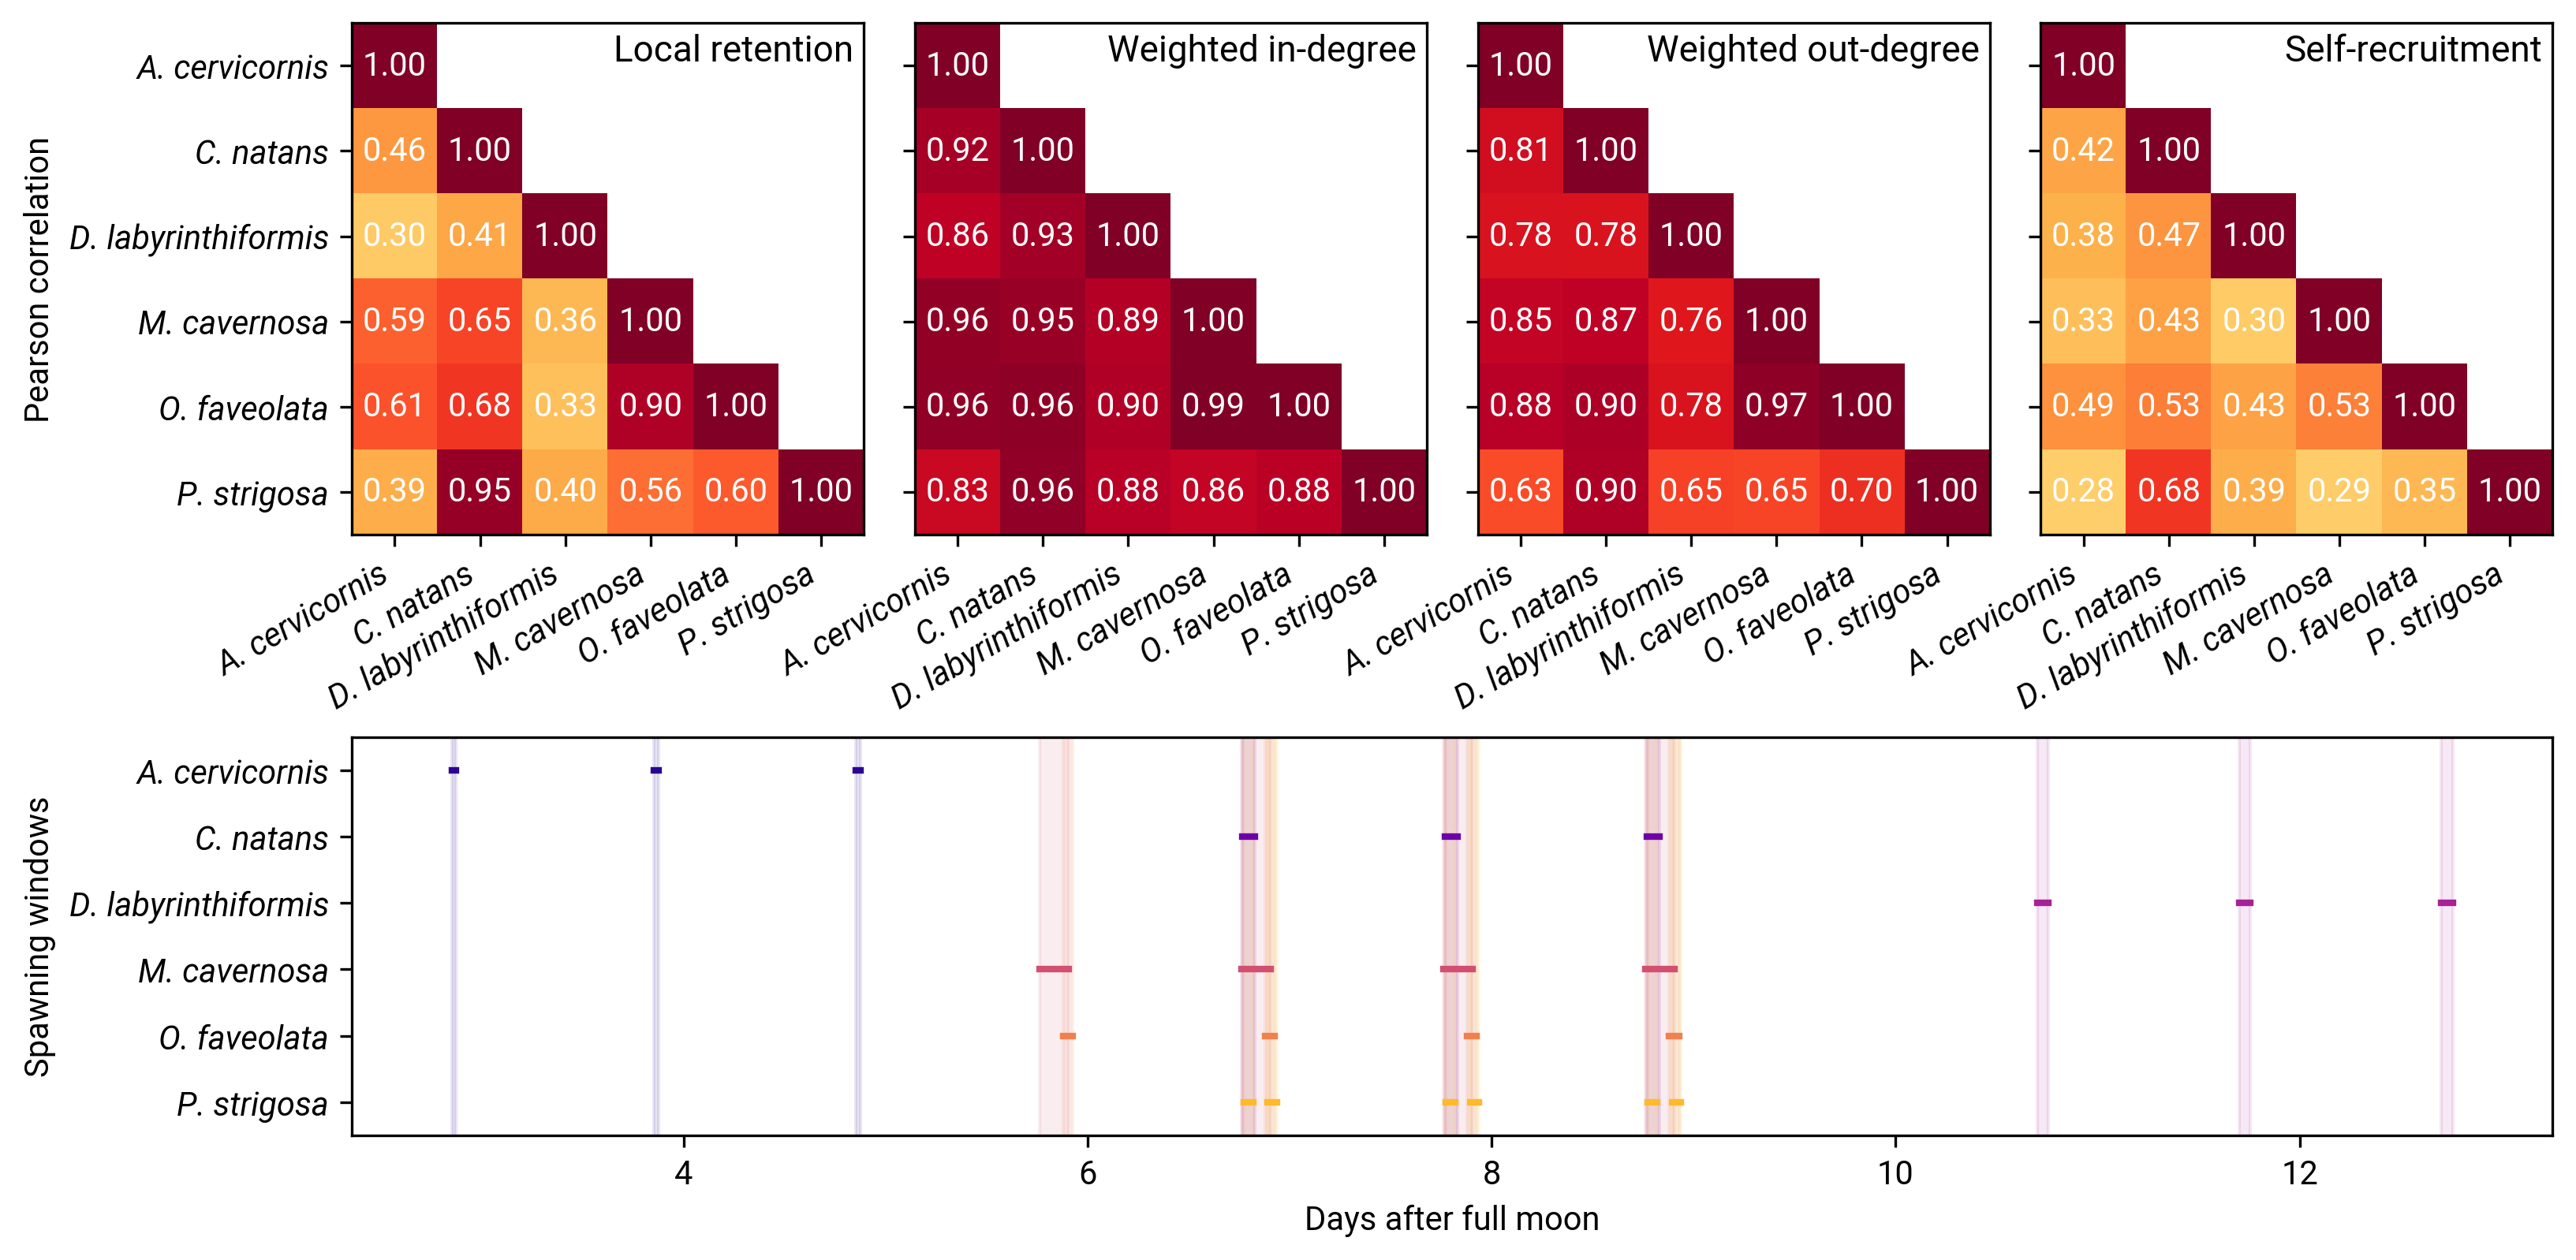
\includegraphics[width=\textwidth]{figures/fig_correlation.png}
    \caption{\textbf{Top}: Pearson correlations of the distributions of local retention, weighted in-degree and out-degree, and self-recruitment for all pairs of species. \textbf{Bottom}: Spawning windows of all coral species in days after full moon. Dlab was not included in the bottom figure, as it spawns in April-May, while all other species spawn in July-August. Connectivity indicators are more strongly correlated between species with similar spawning windows}\label{fig:correlation}
\end{figure}

Clusters of top-performers in terms of local retention were found in the Dry Tortugas, north of the Marquesas, in the Upper Keys, and in the northern Broward-Miami and Deerfield  (Fig. \ref{fig:top10}A). Top performers in terms of weighted in-degree were found in the northern part of Florida's Coral Reef (above latitude 25.6) and in the Dry Tortugas (Fig. \ref{fig:top10}B). Top-performers in terms of weighted out-degree were found in the Dry Tortugas, Biscayne, Broward-Miami regions (Fig. \ref{fig:top10}C). However, there was no clear cluster of bottom-performers in terms of self-recruitment, although most of them were found in the Lower Keys, and Biscayne, Broward-Miami and North Palm Beach regions (Fig. \ref{fig:top10}D). When combining the above-described frequencies, reefs with great restoration potential were found in the Dry Tortugas and norther Broward-Miami, and more marginally in the Middle Keys and North and South Palm Beach (Fig. \ref{fig:top10}E).

\begin{figure}
   \centering
   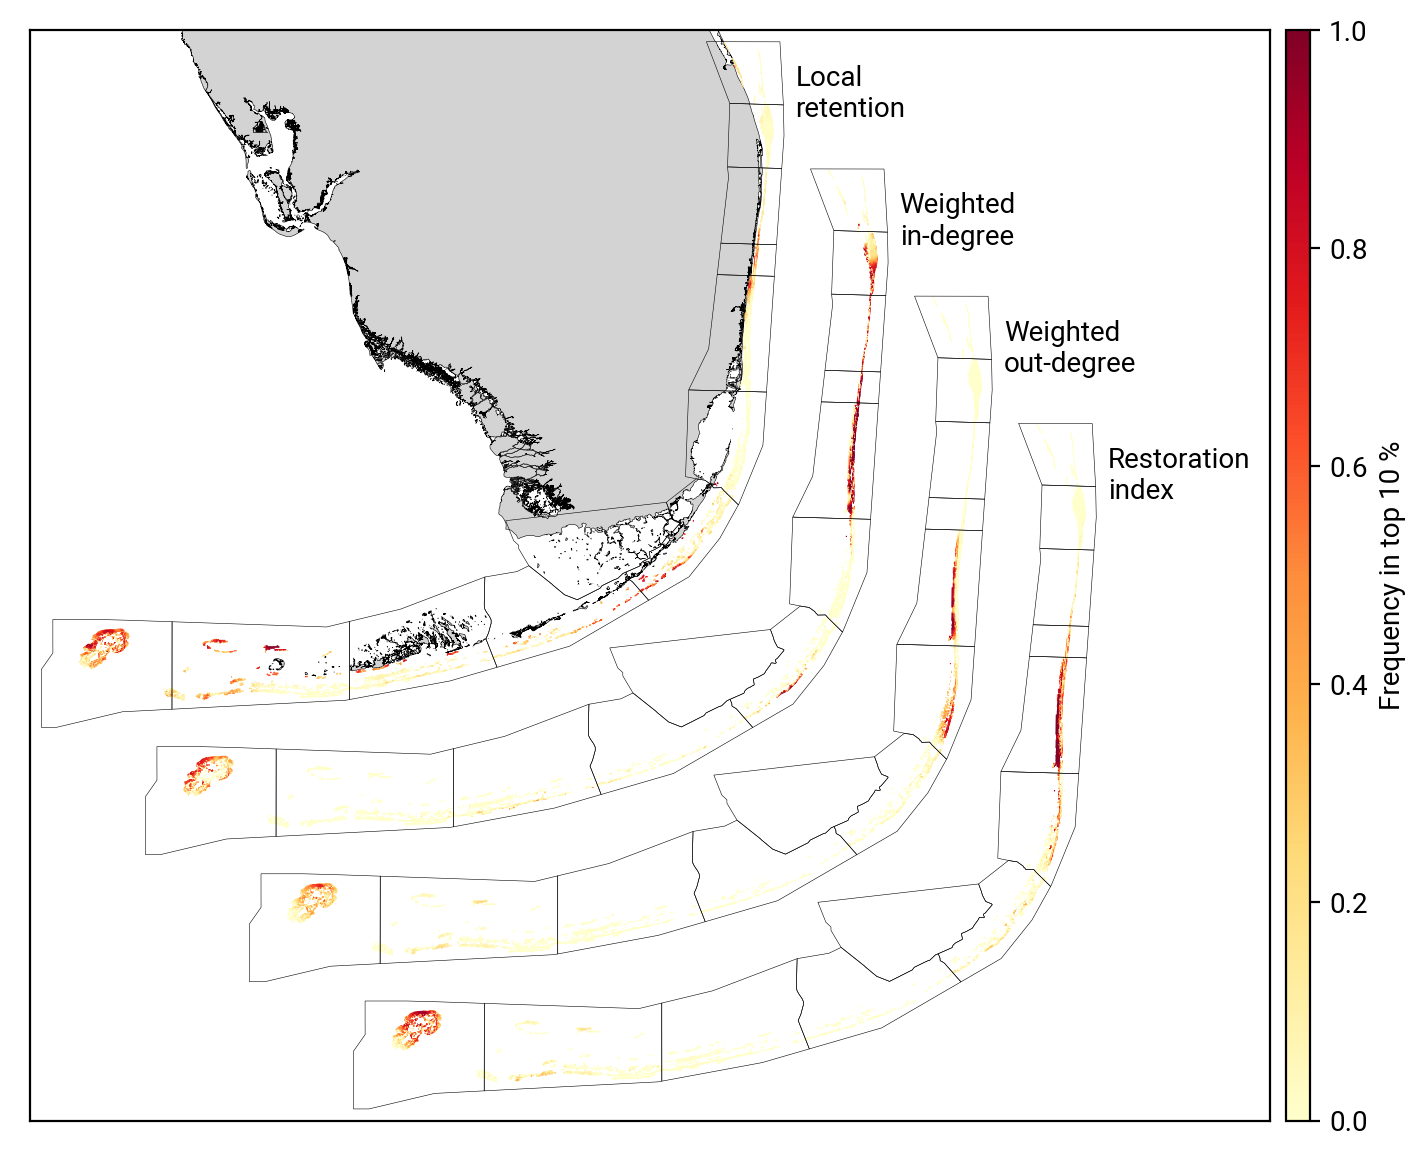
\includegraphics[width=0.95\textwidth]{figures/fig_top10.png}
   \caption{Species-averaged frequency of reefs in the top 10\% yearly values for \textbf{(A)} local retention, \textbf{(B)} weighted in-degree and \textbf{(C)} weighted out-degree. The species-averaged frequency of reefs in flop 10\% yearly values for self recruitment is shown in panel \textbf{(D)}. By multiplying these frequencies, we obtain a combined restoration indicator whose top values correspond to reefs that are top performers of weighted out-degree, in-degree and local retention, and low-performers of self-recruitment, as shown in panel \textbf{(E)}. Reefs with a restoration indicator of 0 are shown in black}\label{fig:top10}
\end{figure}

Self-recruitment exhibited the largest inter-annual variability, with large values of quartile coefficients of dispersion on most reefs. This is consistent with the absence of clear clusters of bottom-performers in terms of self-recruitment. Local retention varied significantly through time as well, except in the Marquesas, Biscayne, and North Palm Beach, where smaller quartile coefficients of dispersion were found. Most reefs showed limited inter-annual variability of weighted in- and out-degrees, except in the Dry Tortugas and Marquesas. Larger values of the quartile coefficient of dispersion were also found in North Palm Beach and the Lower Keys in the case of weighted out-degree.
\begin{figure}
    \centering
    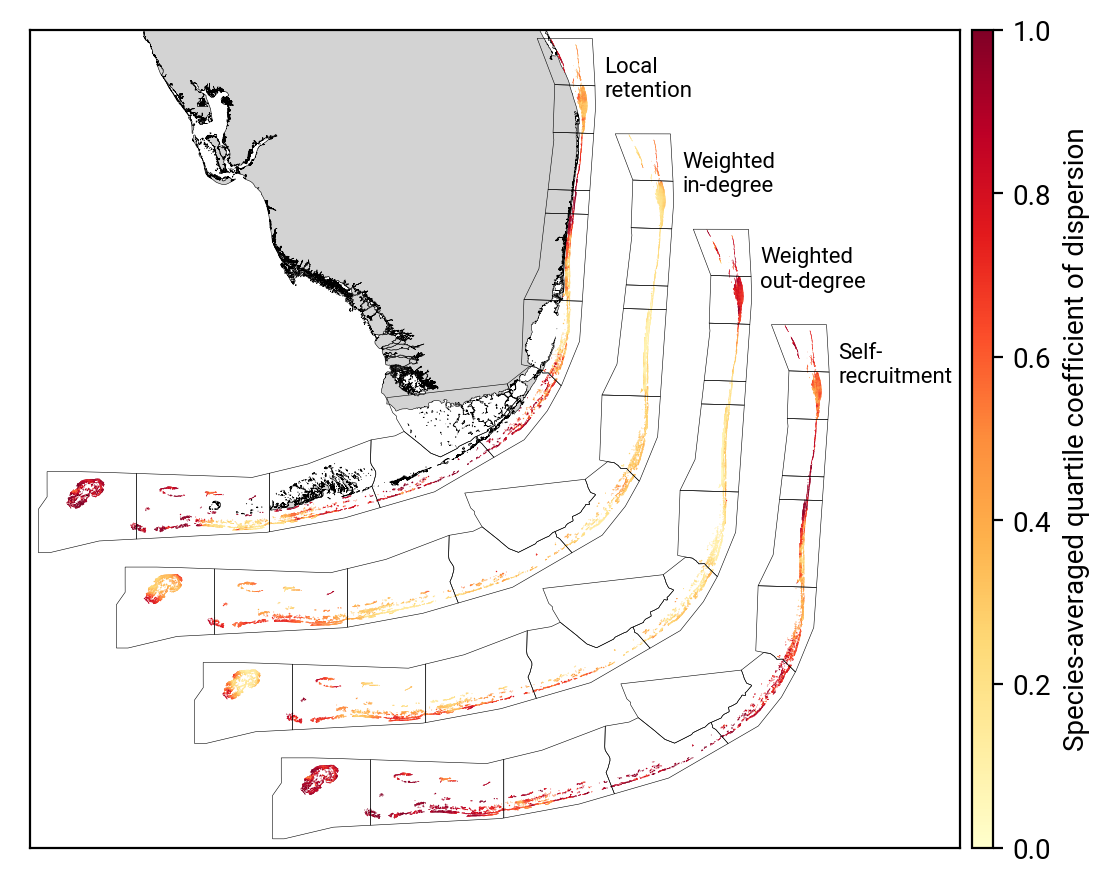
\includegraphics[width=\textwidth]{figures/species_averaged_quartile_coefficient_of_dispersion.png}
    \caption{Species-averaged quartile coefficient of dispersion of the four selected indicators. Weighted in- and out-degrees only exhibited significant inter-annual variability in some parts of FCR, while significant inter-annual variability in terms of local retention and self-recruitment was observed on most reefs.}\label{fig:variability}


\end{figure}

The structure and composition of the SCCs evolved through time for each simulated species (Fig. \ref{fig:scc}). \textit{A.~cervicornis}, \textit{M.~cavernosa} and \textit{O.~faveolata} exhibited the least stable SCC structure, as they yield the weakest number of reef pairs found in the same SCC during all 10 simulated year, with Ofav having the least stable SCC structure. The largest number of reef pairs found in the same SCC during all 10 simulated years was observed in the connectivity network of \textit{D.~labyrinthiformis}, suggesting that this species had the most stable SCC structure. A comparison of the SCC composition of \textit{O.~faveolata} and \textit{D.~labyrinthiformis} in 2017 and 2018 is shown in Fig. \ref{fig:scc}. While most of the SCC structure is conserved between those two years for \textit{D.~labyrinthiformis}; strong structural differences are observed for \textit{O.~faveolata}, especially in the Middle Keys and the Dry Tortugas. Nonetheless, some reefs were consistently found in the same communities for all simulated species and years. These reefs are located in the northern Dry Tortugas, north of the Marquesas, and in the Upper Keys.

\begin{figure}
    \centering
    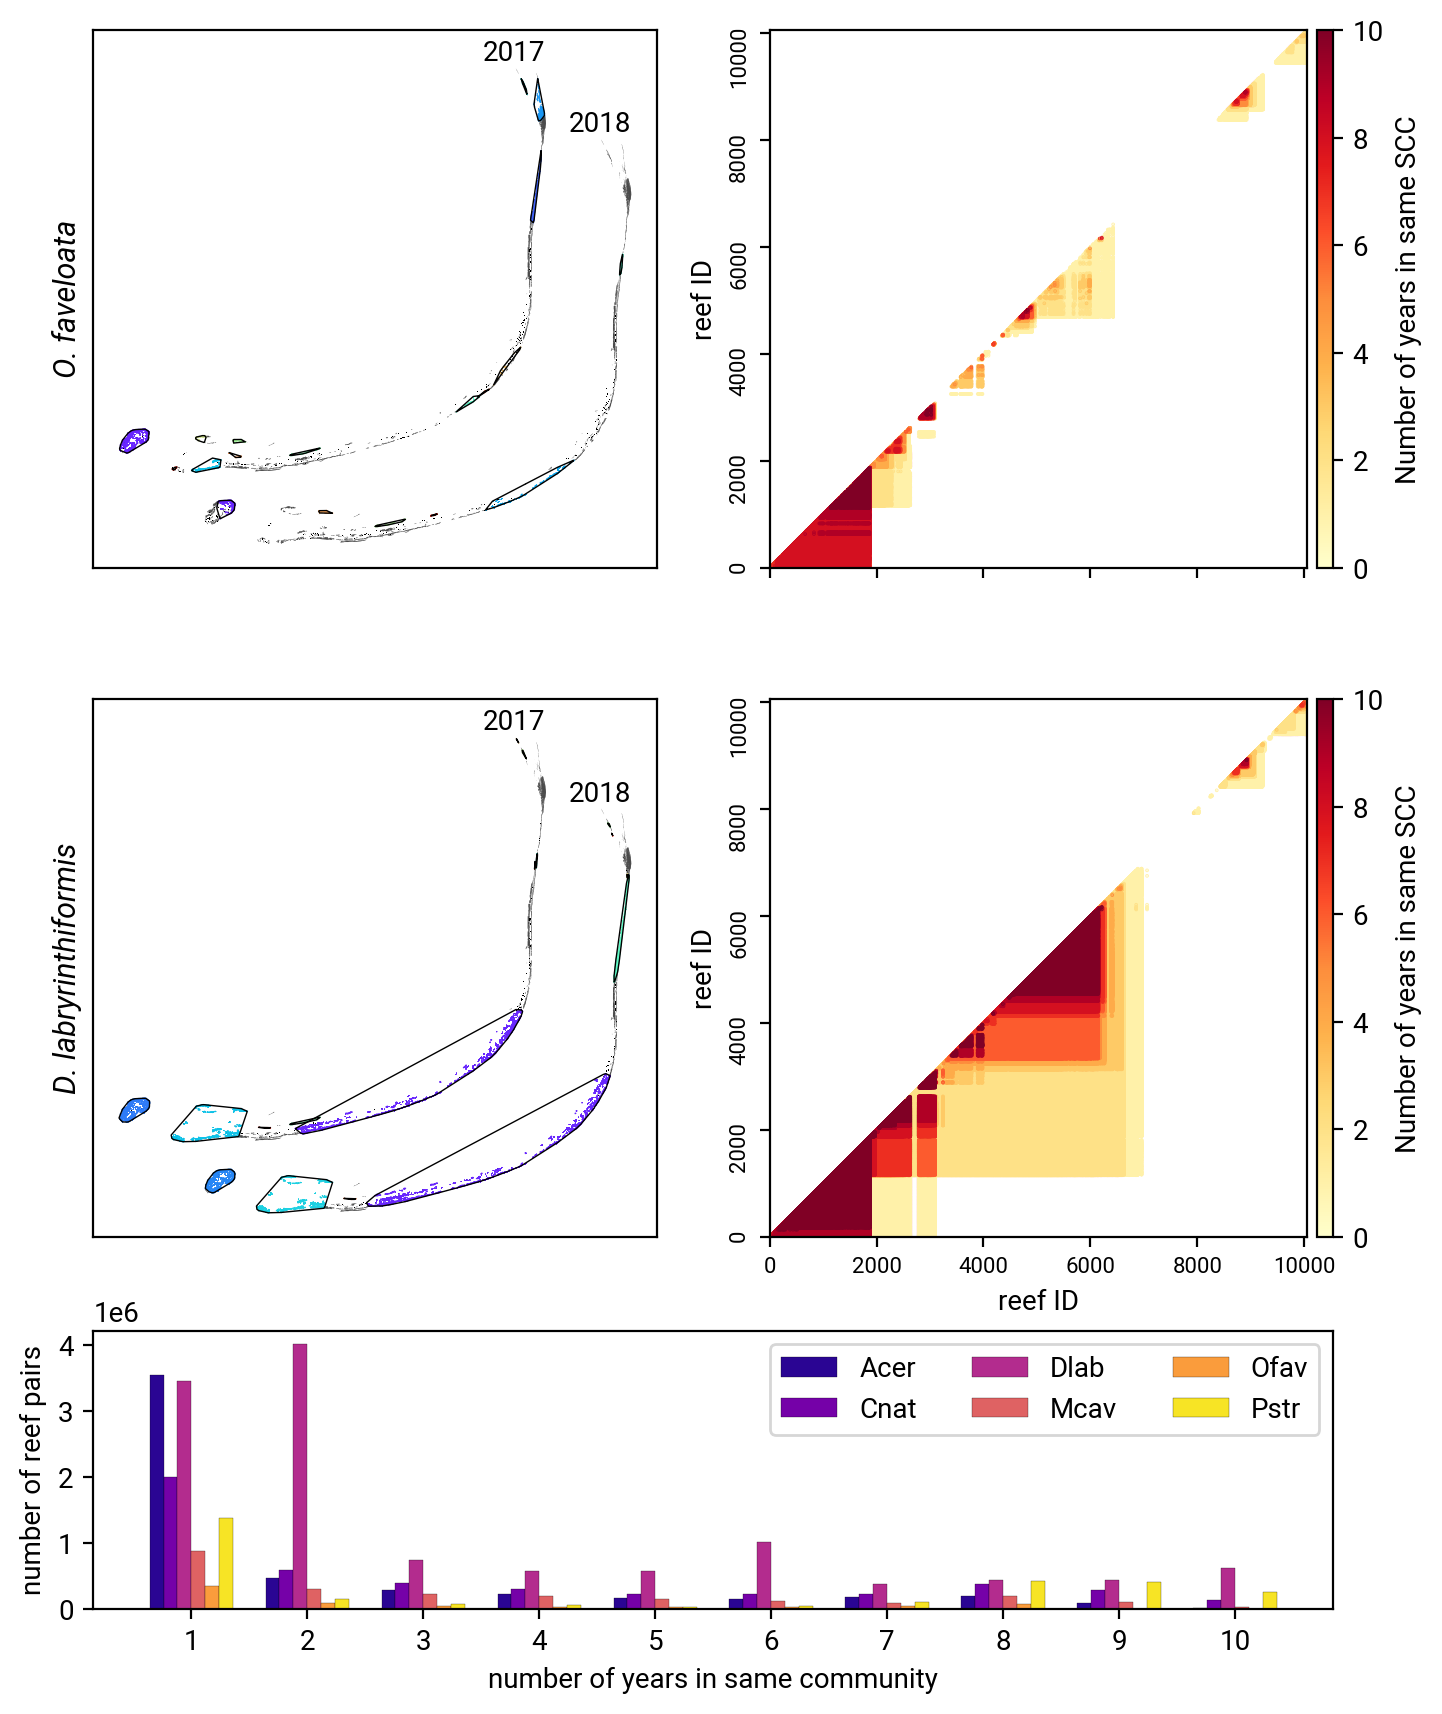
\includegraphics[width=.9\textwidth]{figures/comparison_sccs.png}
    \caption{SCCs of the connectivity networks of \textit{O. faveolata} (\textbf{top}), and \textit{D.~labyrinthiformis} (\textbf{middle}) in 2017 and 2018, and the symmetrical matrix counting the number of simulated years during which each pair of reefs was found in the same SCC for these 2 species. Reefs are ordered according to their geographical coordinates. Reefs of the bottom left (resp. top right) of the matrix correspond to reefs located in the south-west (resp. north east) of Florida's Coral Reef. \textbf{Bottom}: Number of reef pairs found in the same SCC vs. the number of simulated years during which they were found in the same community for each modeled coral species. The connectivity networks of \textit{D.~labyrinthiformis} and \textit{P.~strigosa} exhibit larger more stable communities compared to \textit{O.~faveolata} and \textit{M.~cavernosa}}\label{fig:scc}
\end{figure}

% === DISCUSSION ===

\section*{Discussion}

% Summary of the results
Inter-annual variability of weighted in- and out-degrees for each reef, proxies for respectively source and sink reefs, is limited for most reefs which suggests management planning based on connectivity will be effective. Local retention (a measure of self-persistence) and  self-recruitment (a measure of isolation) vary widely between years. Inter-species variability in connectivity patterns is less pronounced among species which spawn around the same time and have similar egg sizes, however several reefs were identified as good “sources” for all species, and thus constitute optimal sites for protection and/or restoration. Specifically, reefs with great restoration potential were found in the Dry Tortugas and norther Broward-Miami, and more marginally in the Middle Keys and North and South Palm Beach.

% Potential for (coupled) restoration and protection
\emphc{For restoration we can consider source reefs as good places to outplant corals, but also to establish spawning hubs, i.e. areas where corals from different sites are moved to a smaller area (ideally a source reef) to be in close proximity and thus, when they spawn, maximize chances of successful fertilization (i.e. reduce Allee Effects)}

\textbf{Paragraph idea:} Explain the location of some top/bottom-performers based on hydro. \emphc{Please discuss why Dry Tortugas and Marquesas are outliers... this was already obvious in \cite{king2023larval}}

\textbf{Paragraph idea:} The importance of inter-annual variability of the connectivity indicators

% Inter-specific variability
The inter-specific variability in larval survivals and competency dynamics also explains the inter-specific variability in connectivity patterns. For all species, larval survival decreased over time for all species (Figure X, Table Y) because coral larvae are mainly lecithotrophic and thus their energy reserves slowly become exhausted resulting in eventual death. It remains to be determined if the recorded rates of larval mortality are species-specific and/or driven by parental genotype, history of stress exposure, food quantity and quality they had access to, and/or symbiont community \citep{jones2011tradeoffs, baums2013genotypic, padilla2013all, kirk2018genomic}. The estimated rates of acquisition (a) and loss of competency (b) also differed between species (Table \ref{tab:species}). For some species, the proportion of larvae that settled was quite low (Fig. \ref{fig:top10}), thus is possible that the crustose coralline algae and microbial biofilm used to induce settlement were not as adequate for them. However, the species that displayed lower settlement, \textit{P.~strigosa}, also registered the highest mortality suggesting that rather than species-specific, rates of mortality, and acquisition and loss of competency are mostly explained by parental condition. The interspecific differences in the minimum time to competency are unequivocally species-specific, and mostly explained by their egg size \citep{figueiredo2013synthesizing}. As egg size (and ratio of the surface-area to the volume) increases, the elimination of CO2 (which is toxic) from the embryo surface is progressively harder, reducing the pace of larval development \citep{berrill1935cell, einum2002egg}.

\textbf{Paragraph idea:} Importance of robust connectivity estimates to optimize coral restoration in regard to establishment of networks of marine protected areas and optimal/most effective restoration

\textbf{Paragraph idea:} Limitations of the study: 2D model $+$ Potential connectivity $\rightarrow$ habitat suitability and post-settlement survival not considered $+$ we assumed a uniform coral cover over all reefs by lack of information


% === CONCLUSION ===
\section*{Conclusion}

\lipsum[1-1]

% === Lots of stuff ===

\section*{Data availability}

TBD.
% The datasets generated during the current study are available from the corresponding author on reasonable request.

\section*{Code availability}

The \slim source code can be found at \href{https://git.immc.ucl.ac.be/slim/slim}{https://git.immc.ucl.ac.be/slim/slim}.

\section*{Acknowledgements}

Computational resources have been provided by the supercomputing facilities of the \textit{Universit\'e catholique de Louvain} (CISM/UCLouvain) and the \textit{Consortium des \'Equipements de Calcul Intensif en F\'ed\'eration Wallonie Bruxelles} (CECI) funded by the \textit{Fonds de la Recherche Scientifique de Belgique} (F.R.S.-FNRS) under convention 2.5020.11. Thomas Dobbelaere is a postdoctoral researcher supported by the F.R.S-FNRS.

\section*{Author contributions statement}

TBD.

\section*{Competing interests}

The authors declare no competing interests.

%  === REFERENCE ===

\bibliographystyle{elsarticle-harv}
\bibliography{biblio.bib}
\newpage
\appendix

\section{Invariant component of the SCCs}

\begin{figure}[h!]
    \centering
    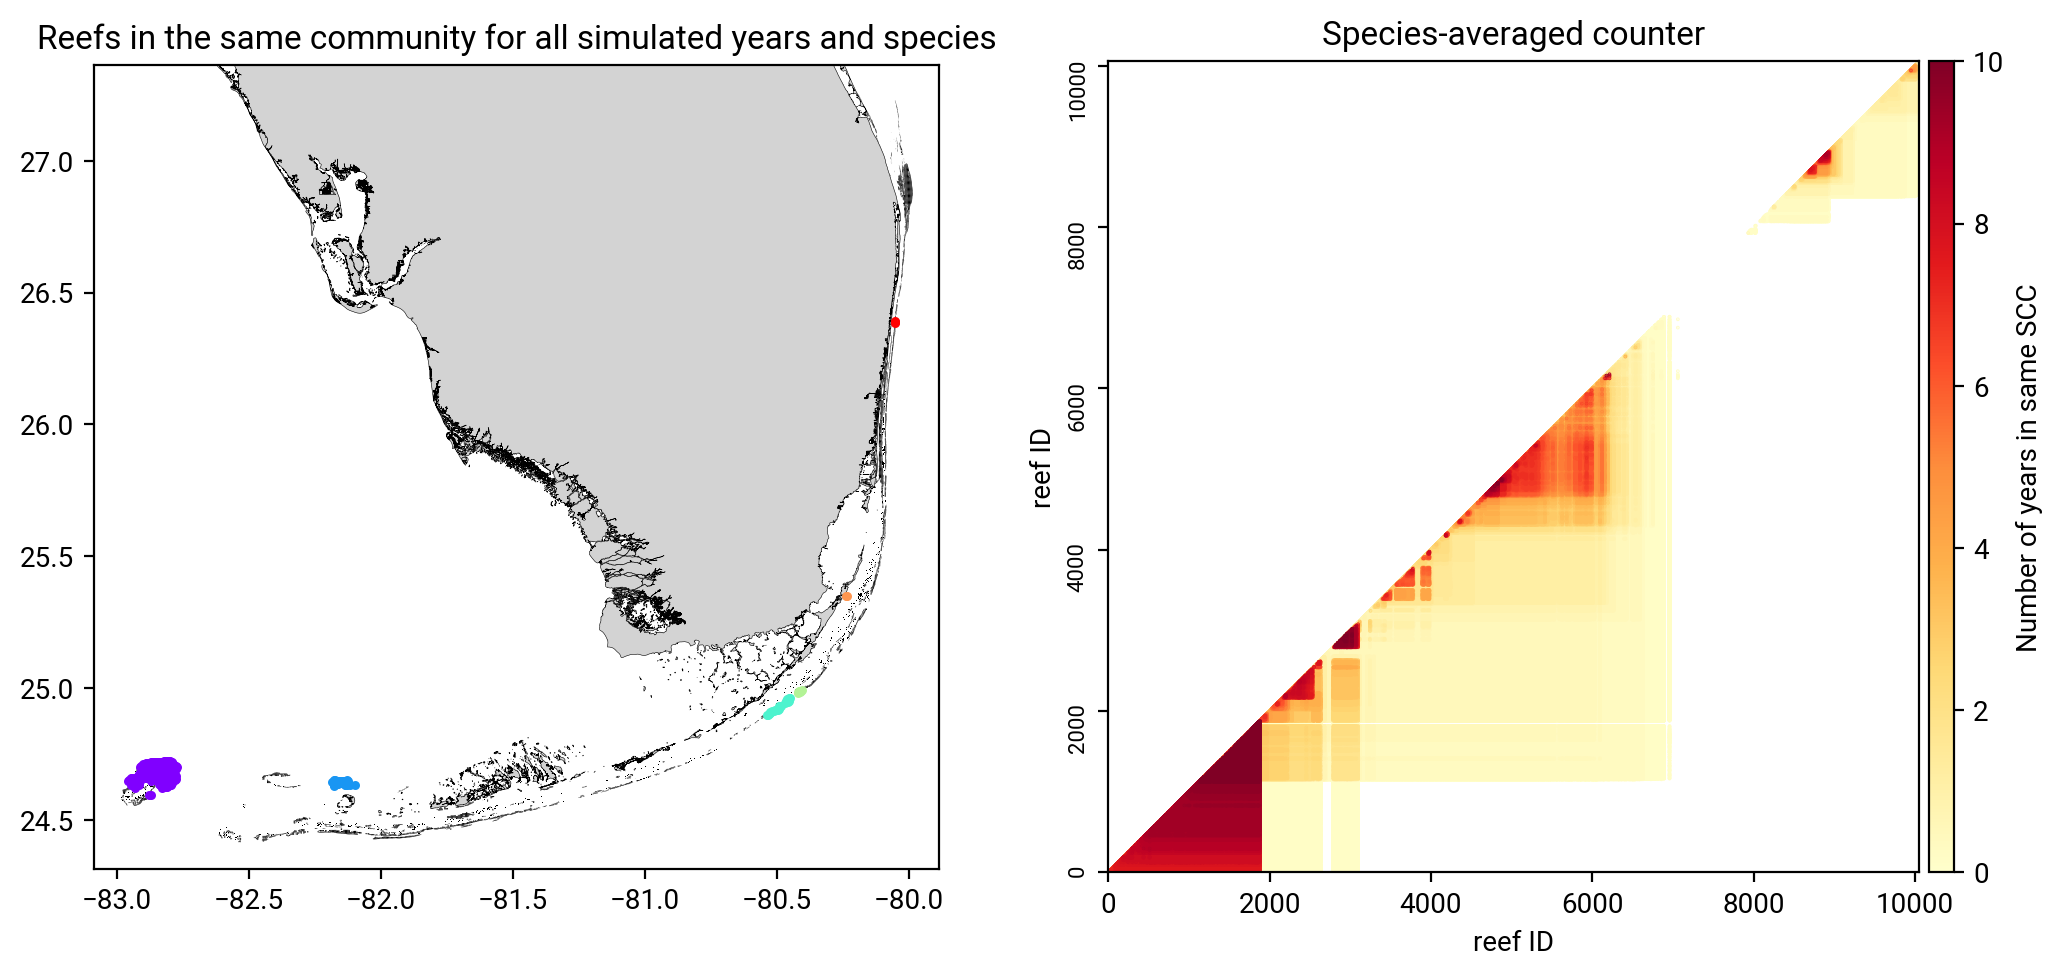
\includegraphics[width=\textwidth]{figures/mean_counter.png}
    \caption{Reefs in the same SCC for all simulated years and species}\label{fig:mean_counter}
\end{figure}

\begin{figure}
    \centering
    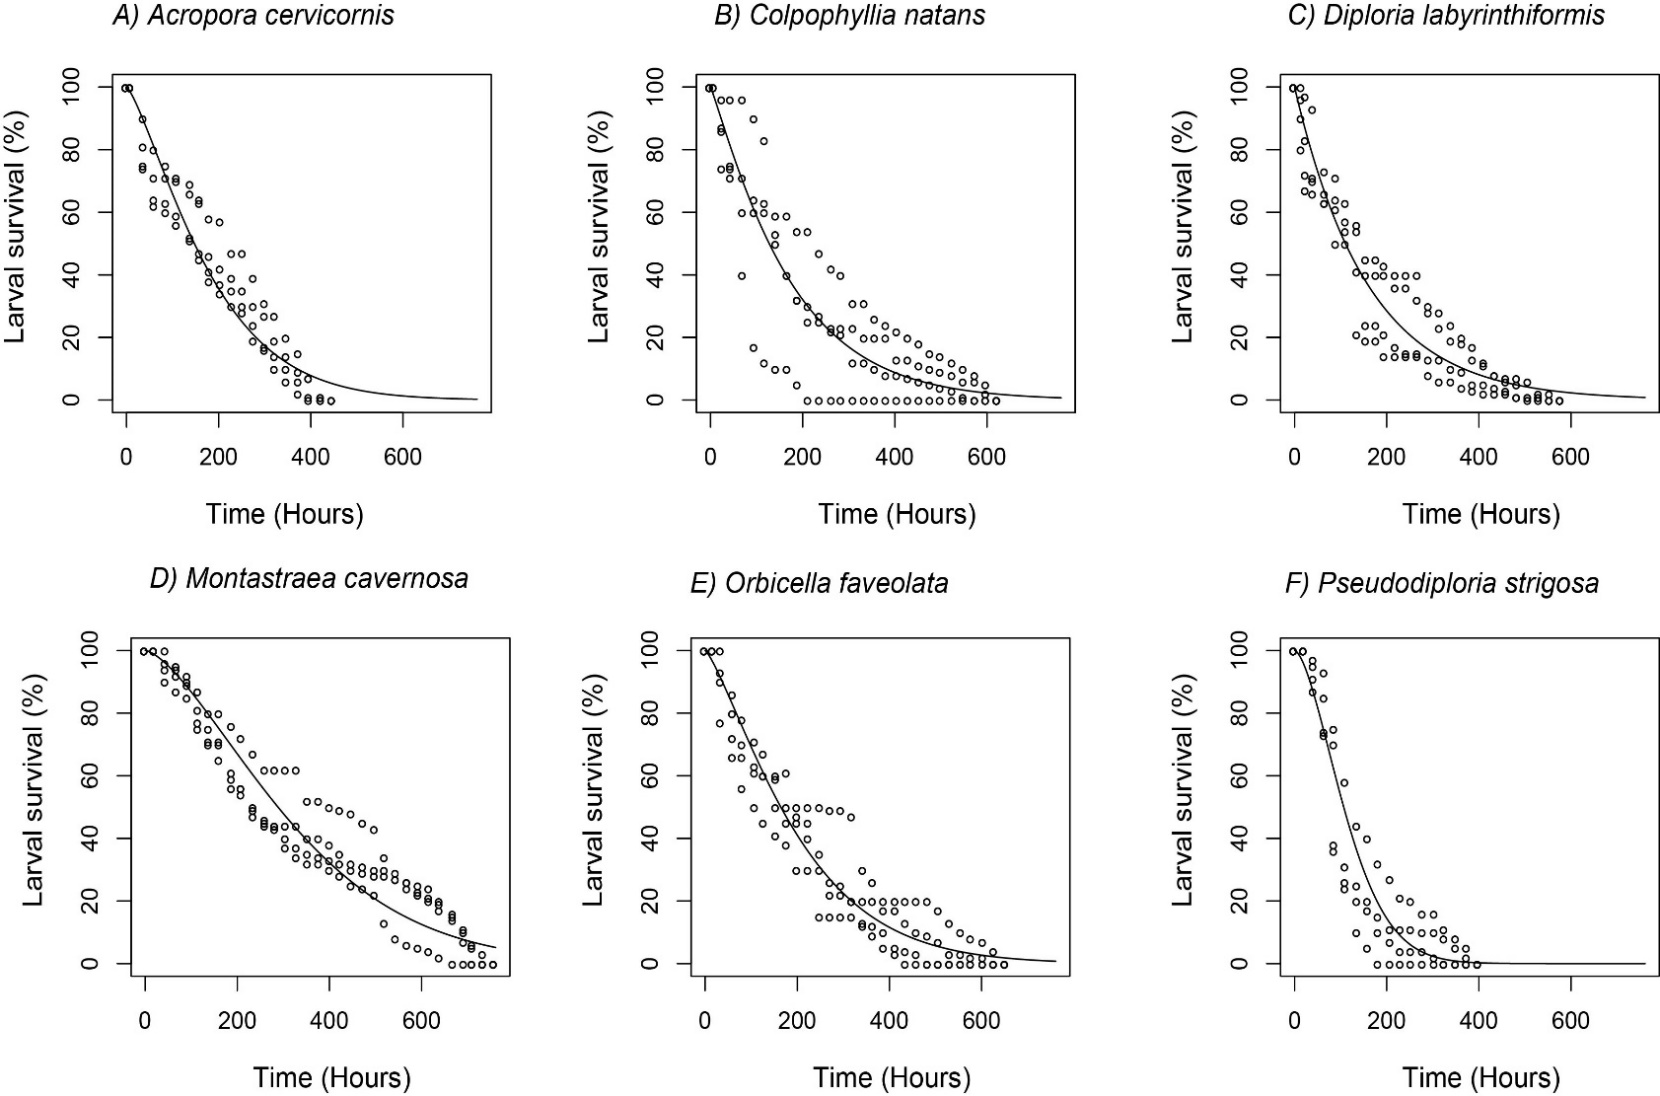
\includegraphics[width=\textwidth]{figures/fig_mortality.jpeg}
    \caption{ Percent larvae alive over time for the six Caribbean coral species studied. A) \textit{A.~cervicornis}, B) \textit{C.~natans}, C) \textit{D.~labyrinthiformis}, D) \textit{M.~cavernosa}, E) \textit{O.~faveolata}, and F) \textit{P.~strigosa}. Circles represent the observations, and lines the best fitted model. The model of best fit for shape of mortality of all species was the standard Weibull model except for \textit{D.~labyrinthiformis}, which mortality was best fit with an exponential model}\label{fig:mortality}
\end{figure}
\begin{figure}
    \centering
    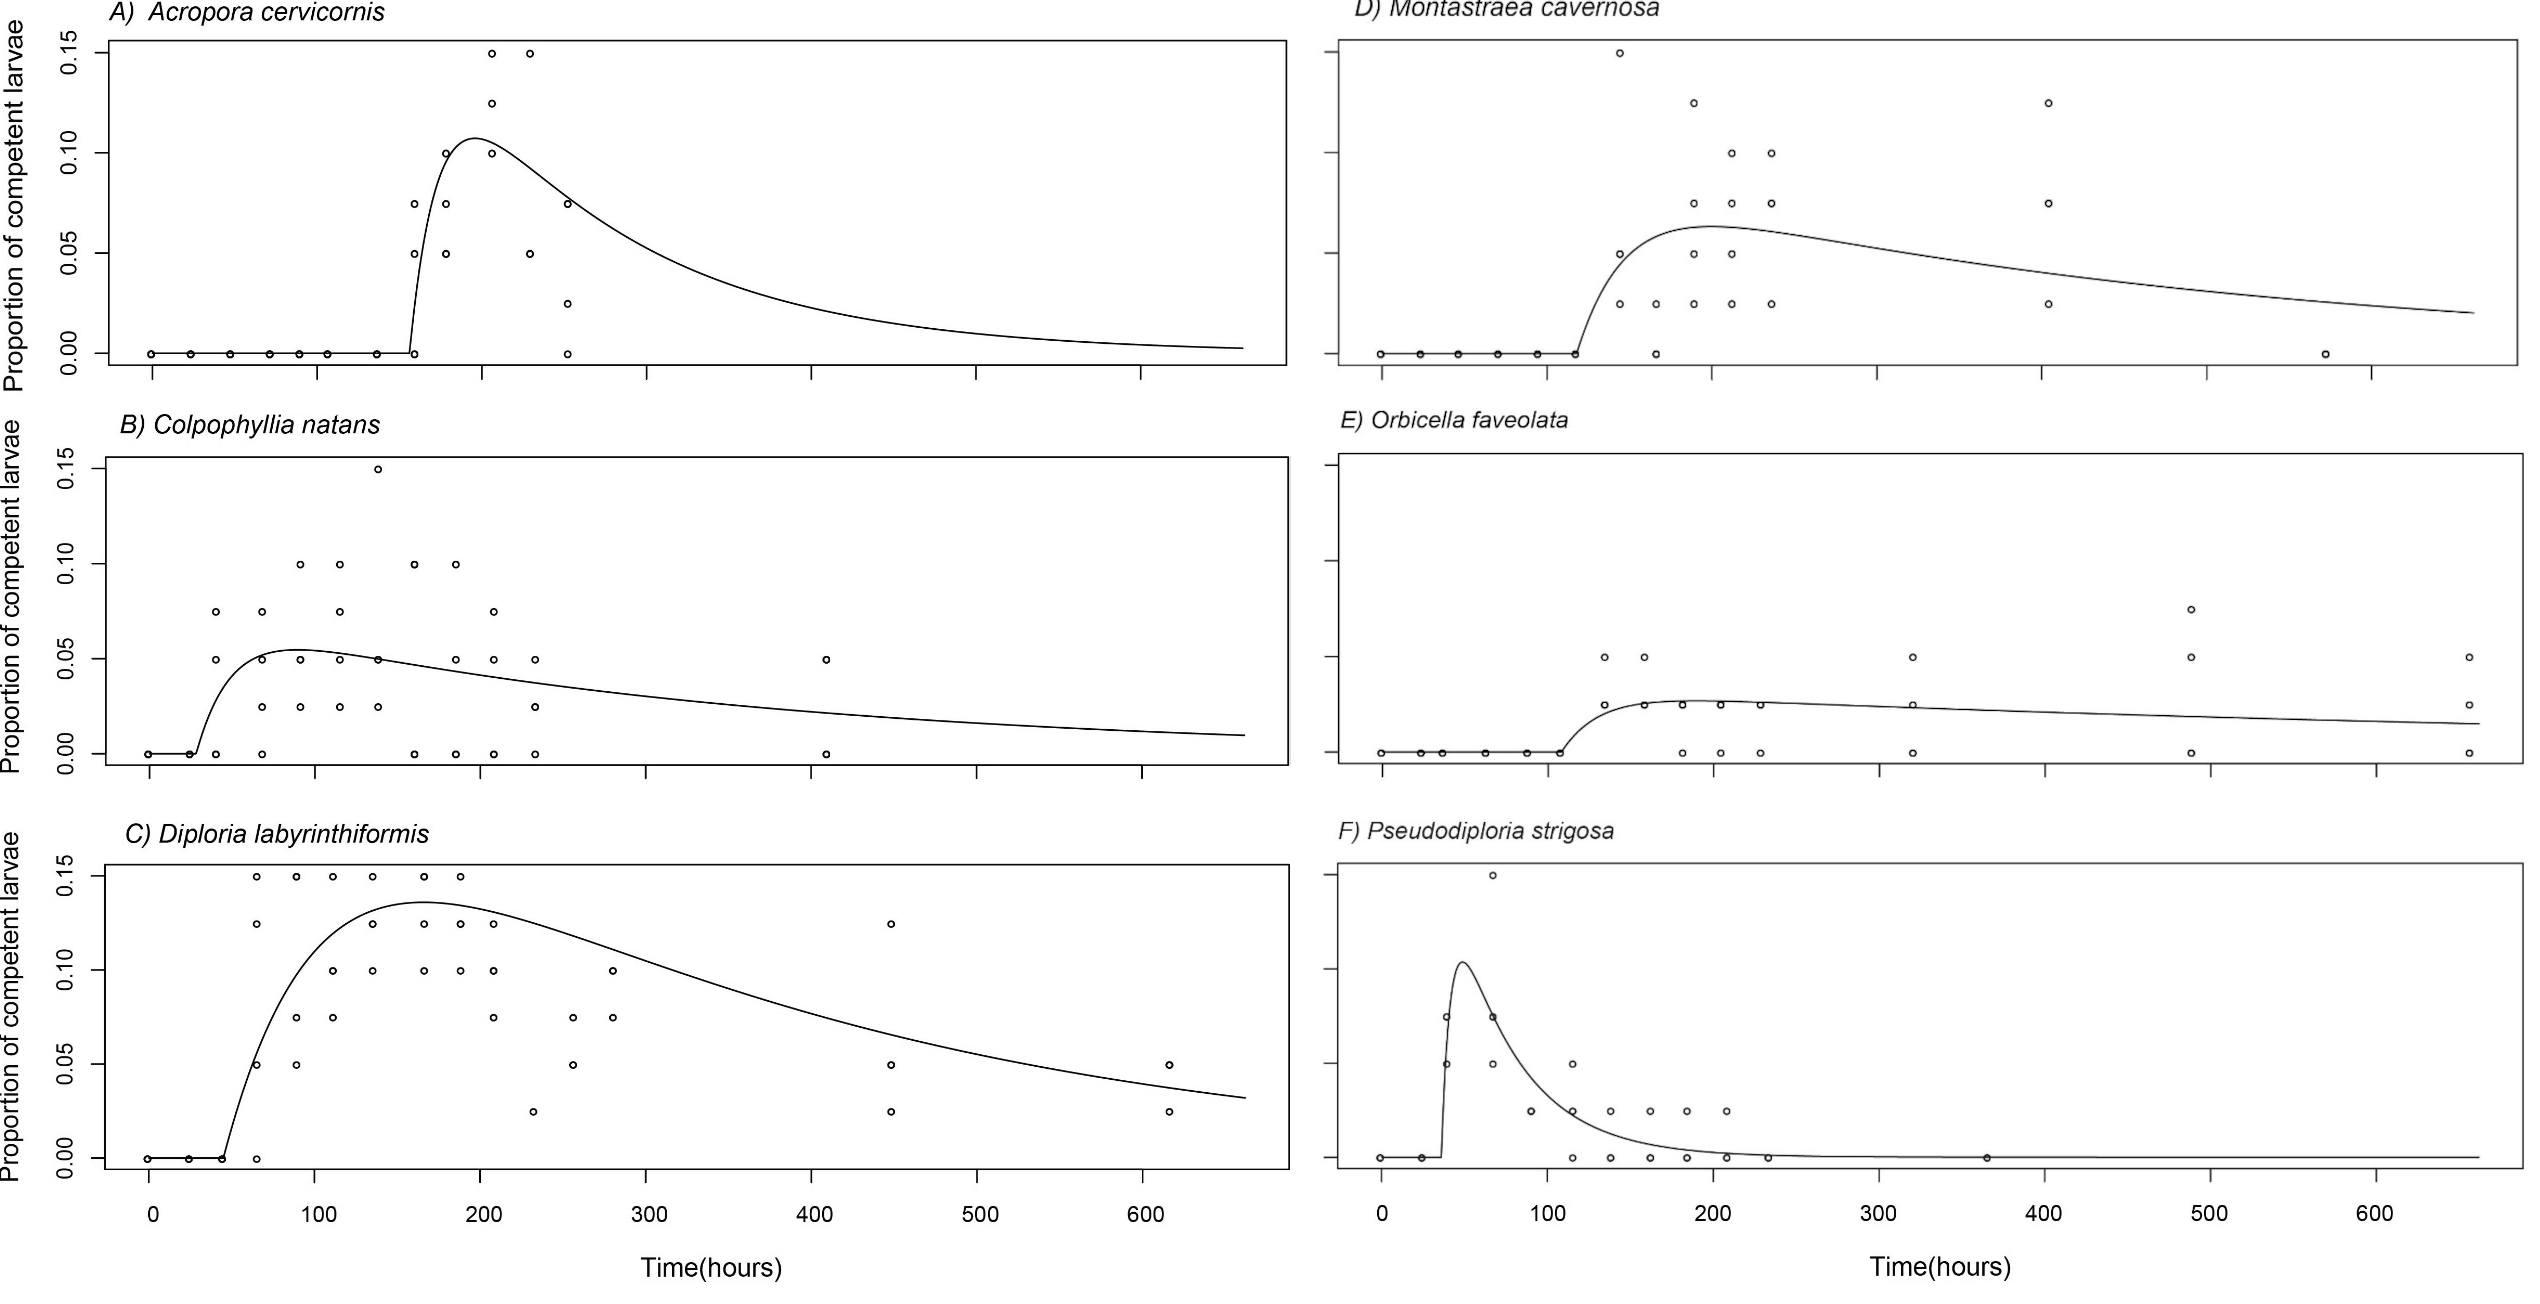
\includegraphics[width=\textwidth]{figures/fig_competence.png}
    \caption{Proportion of competent larvae over time for the six species studied. A) \textit{A.~cervicornis}, B) \textit{C.~natans}, C) \textit{D.~labyrinthiformis}, D) \textit{M.~cavernosa}, E) \textit{O.~faveolata}, and F) \textit{P.~strigosa}. The model of best fit for shape of loss of competency of all species was the exponential model.}\label{fig:competence}
\end{figure}

\end{document}
\endinput
